\section{Idea}

\gammasky is a one-stop resource for browsing images and catalogs but also for closely examining a specific gamma-ray source. Although it was mainly built for the greater astronomical community, the webpage additionally targets the general public through a user-friendly interface and a clean information layout, all of which are compiled under cutting-edge web tools.

\begin{figure}[tb]
\centerline{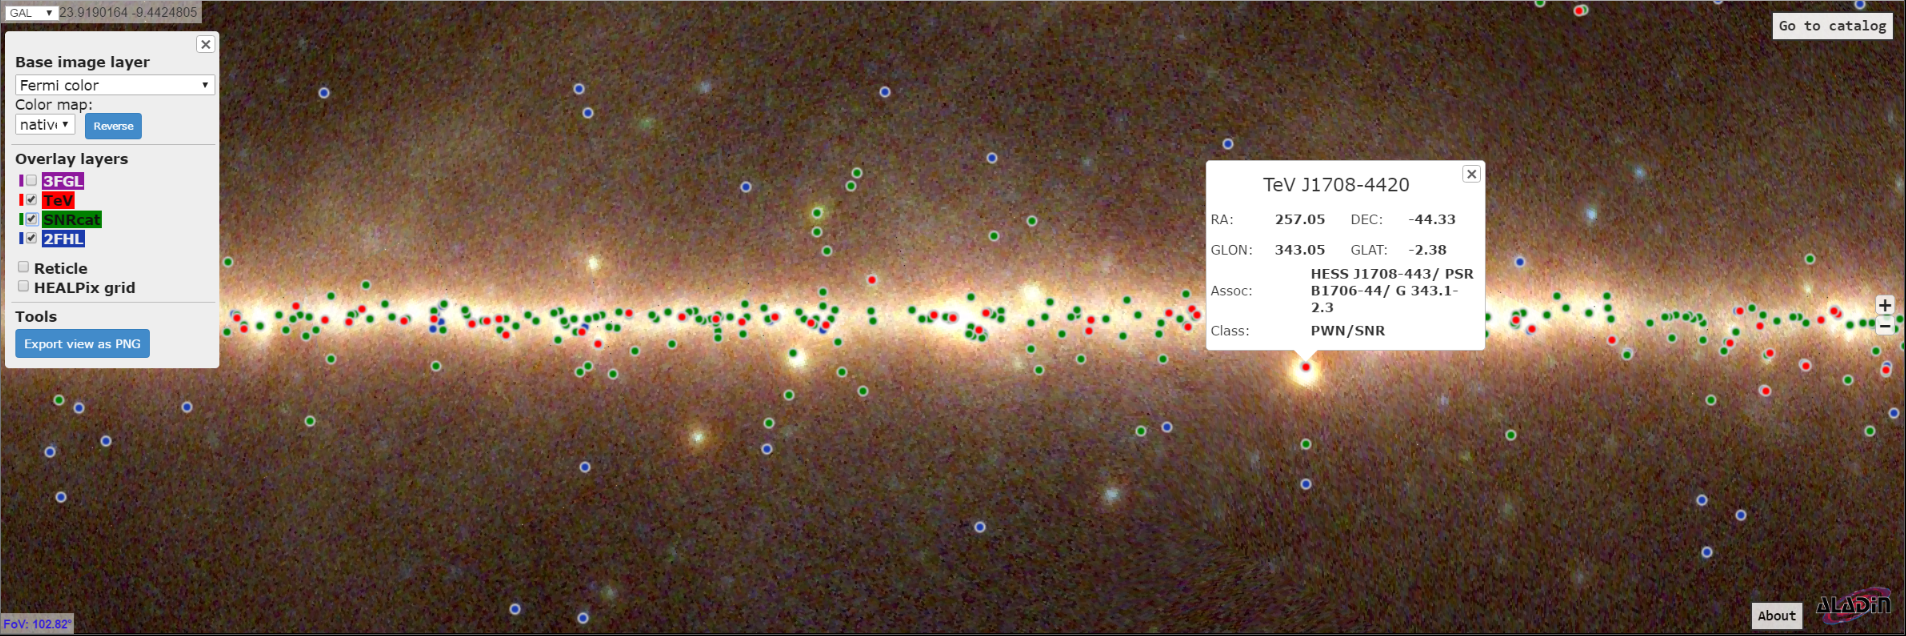
\includegraphics[width=\textwidth]{figures/mapview_wide}}
\caption{Map View of \gammasky showing the gamma-ray sky observed by the space-based Fermi-LAT, broken into three bands: 0.3-1 GeV (red-band), 1-3 GeV (green-band), and 3-300 GeV (blue-band). The pop-up for one TeV source is displayed, as well as the toolbar on the side containing widgets for controlling the map overlays.}
\label{fig:mapview}
\end{figure}

\begin{figure}[tb]
\centerline{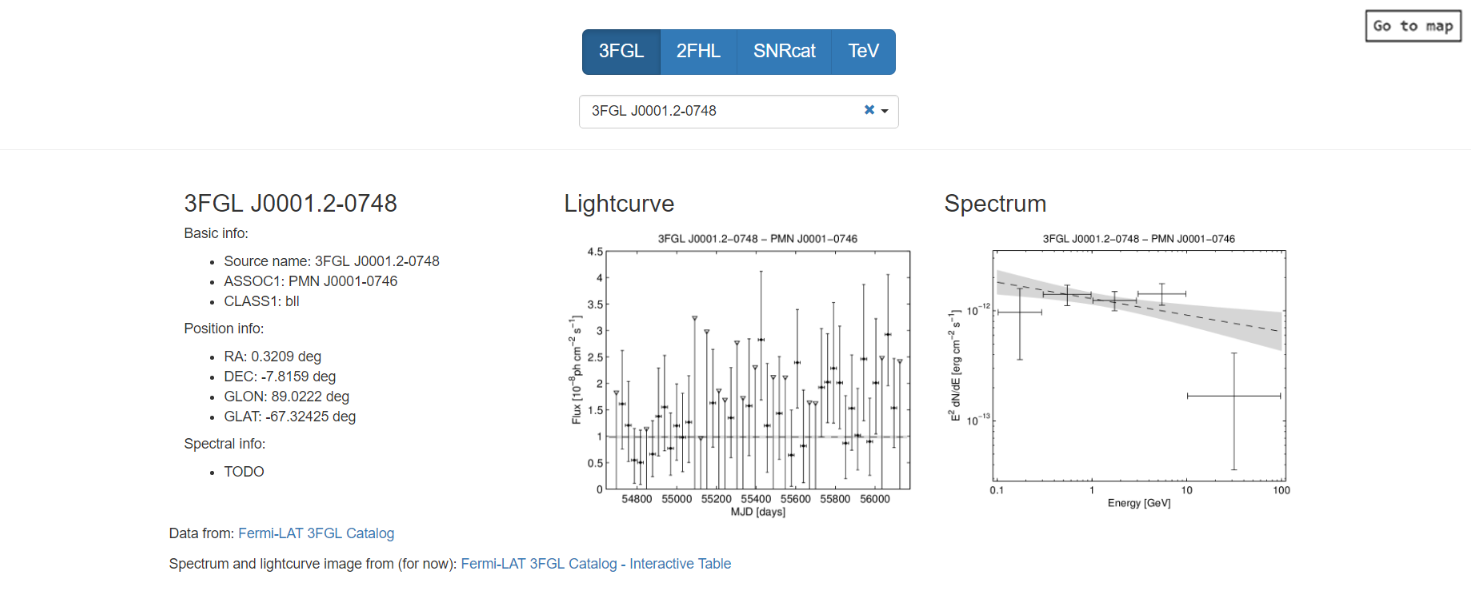
\includegraphics[width=\textwidth]{figures/catview_wide_zoom}}
\caption{Catalog View of \gammasky showing the catalog and source selection fields at the top, and the detailed view for one source from the Fermi-LAT 3FGL catalog.}
\label{fig:catview}
\end{figure}

Individuals who access \url{http://gamma-sky.net} via any modern internet browser will be welcomed with the Map View homepage. This page displays overlays of multi-wavelength survey images, most of which are all-sky, wrapped around a three-dimensional sphere. Gamma-ray sources from our catalog data have then been pinpointed onto the sphere, as shown in Figure~\ref{fig:mapview}. The map features pan-and-zoom functionality for easily navigating and quickly browsing the sky. The Map View page also utilizes a powerful search tool to either pan the view to a given sky position or locate a source by name. This functionality is intended to work similar to Google Maps\footnote[1]{https://www.google.com/maps}, and allows the user to easily find sources of interest and study their visual context. See Table~\ref{tab:images} for our selection of images on the website and Table~\ref{tab:catalogs} for the catalogs we display. \gammasky additionally embodies a Catalog View, which incorporates more detailed information for each of the sources in our catalogs. Professional astronomers will navigate to this component of the website for the deep investigation of a particular source. The Catalog View page is shown in Figure~\ref{fig:catview}.

\begin{table}[bt]

\caption{
Survey images of interest to gamma-ray astronomers available on \gammasky . Note that this is only a very small selection, there are over 300 other multi-wavelength survey images available from CDS via Aladin Lite. The ones listed here were not produced by us specifically for \gammasky . We plan to add more gamma-ray survey images from the GeV energy range (high-energy Fermi-LAT data) and the TeV energy range (H.E.S.S. Galactic plane survey).
}
\label{tab:images}
\tabcolsep7pt\begin{tabular}{ lrlrl }
\hline
Image & Resolution (arcmin) & Type & Band & Coverage\\
\hline
Fermi-LAT & TBD & gamma-ray &  & all-sky\\
AKARI 90um & 1 & infrared &  & all-sky\\
CGPS-VGPS CONT & 1 & radio &  & galactic plane\\
Haslam 408 & 51 & radio & 408 MHz & all-sky\\
IRIS Band 4-100um & TBD & infrared &  & all-sky\\
Planck R1 + R2 HFI & TBD & microwave & 353-545-857 GHz & all-sky\\
Planck R2 LFI & TBD & microwave & 30-44-70 GHz & all-sky\\
Spitzer GLIMPSE360 & 0.02 & infrared &  & galactic plane\\
\multicolumn{5}{c}{300+ other HIPS survey images available from \url{http://aladin.u-strasbg.fr/hips/list}} \\
\hline
\end{tabular}

\end{table}


\begin{table}[bt]

\caption{
Source catalogs currently displayed on \gammasky .
We intend to add additional catalogs of interest to gamma-ray astronomers to the website in the future, including the upcoming H.E.S.S. and HAWC TeV source catalogs, as well as the ATNF Pulsar Catalogue.
}
\label{tab:catalogs}
\tabcolsep7pt\begin{tabular}{ lrll }
\hline
Catalog   & Sources & Updates    & Description \\
\hline
gamma-cat &     153 & continuous & Open TeV gamma-ray source catalog  \\
&&& \gammacat  \\
2FHL      &     360 & fixed      & Second Fermi-LAT catalog of high-energy sources \citep{2fhl}\\
&&& \url{http://fermi.gsfc.nasa.gov/ssc/data/access/lat/2FHL/}  \\
3FGL      &    3034 & fixed      & Third Fermi-LAT point source catalog \citep{3fgl}\\
&&& \url{http://fermi.gsfc.nasa.gov/ssc/data/access/lat/4yr_catalog/}  \\
SNRcat    &     378 & continuous & A census of high-energy observations of Galactic supernova remnants \citep{snrcat}\\
&&& \url{http://www.physics.umanitoba.ca/snr/SNRcat/} \\
\hline
\end{tabular}
\end{table}


\gammasky aims to be a resource for examining a source or region; however, any tools for extended analysis will not be incorporated into the website. Instead for such continued investigation, we point users to Gammapy \cite{gammapy}, a Python package for gamma-ray astronomy, which can used to run scripts locally. These scripts will generate the detailed plots and publication-worthy results that astronomers are interested in. Alternatively, users may navigate to TeVCat \cite{tevcat} for investigating TeV sources, or the ASI Science Data Center (ASDC) website for their online tools (e.g. ASDC Data Explorer\footnote[2]{http://www.asdc.asi.it/tutorial/DataExplorer/DataExplorerTutorial.html}, SED Builder\footnote[3]{http://www.asdc.asi.it/tutorial/SEDBuilder/SEDBuilderTutorial.html}) and their TeGeV Catalogue for TeV sources \cite{tgevcat}.


It is imperative for all of our data on the online portal to be openly available for download and local analysis by any user. Additionally, the website is an entirely open-source project, and other developers are welcome to contribute to the code. We advise those interested in contributing to visit our GitHub repository at \url{https://github.com/gammapy/gamma-sky}.
